\documentclass[../../main.tex]{subfiles}


\begin{document}
\subsection*{(a)}
We can split the event log into two event logs using the plugin 'Filter Log on Event Attribute Values' with the following selections:\\
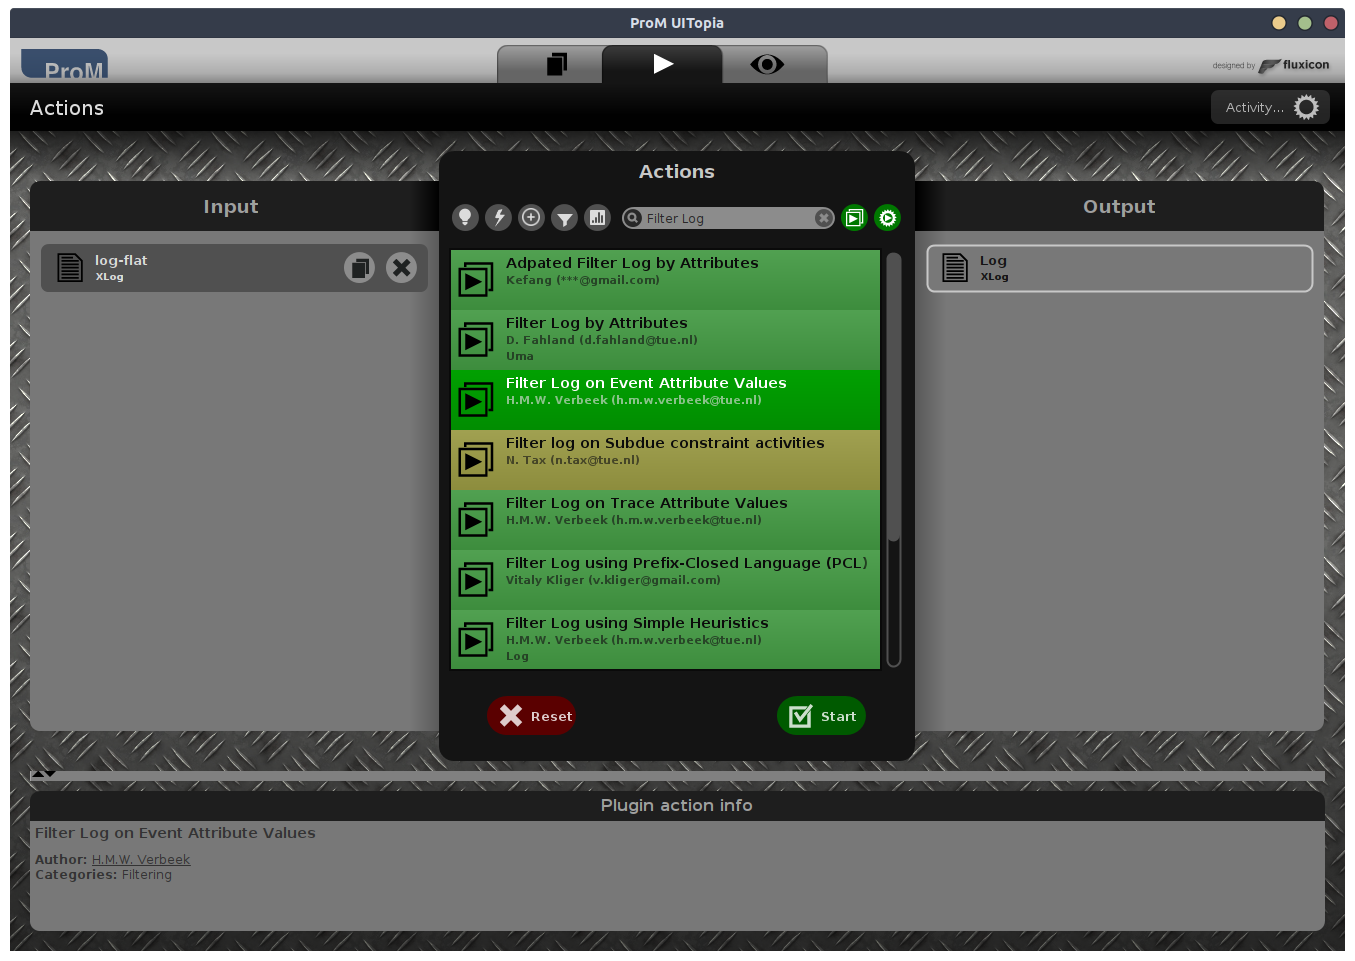
\includegraphics[width=0.33\columnwidth]{img/ProM_a_plugin.png}
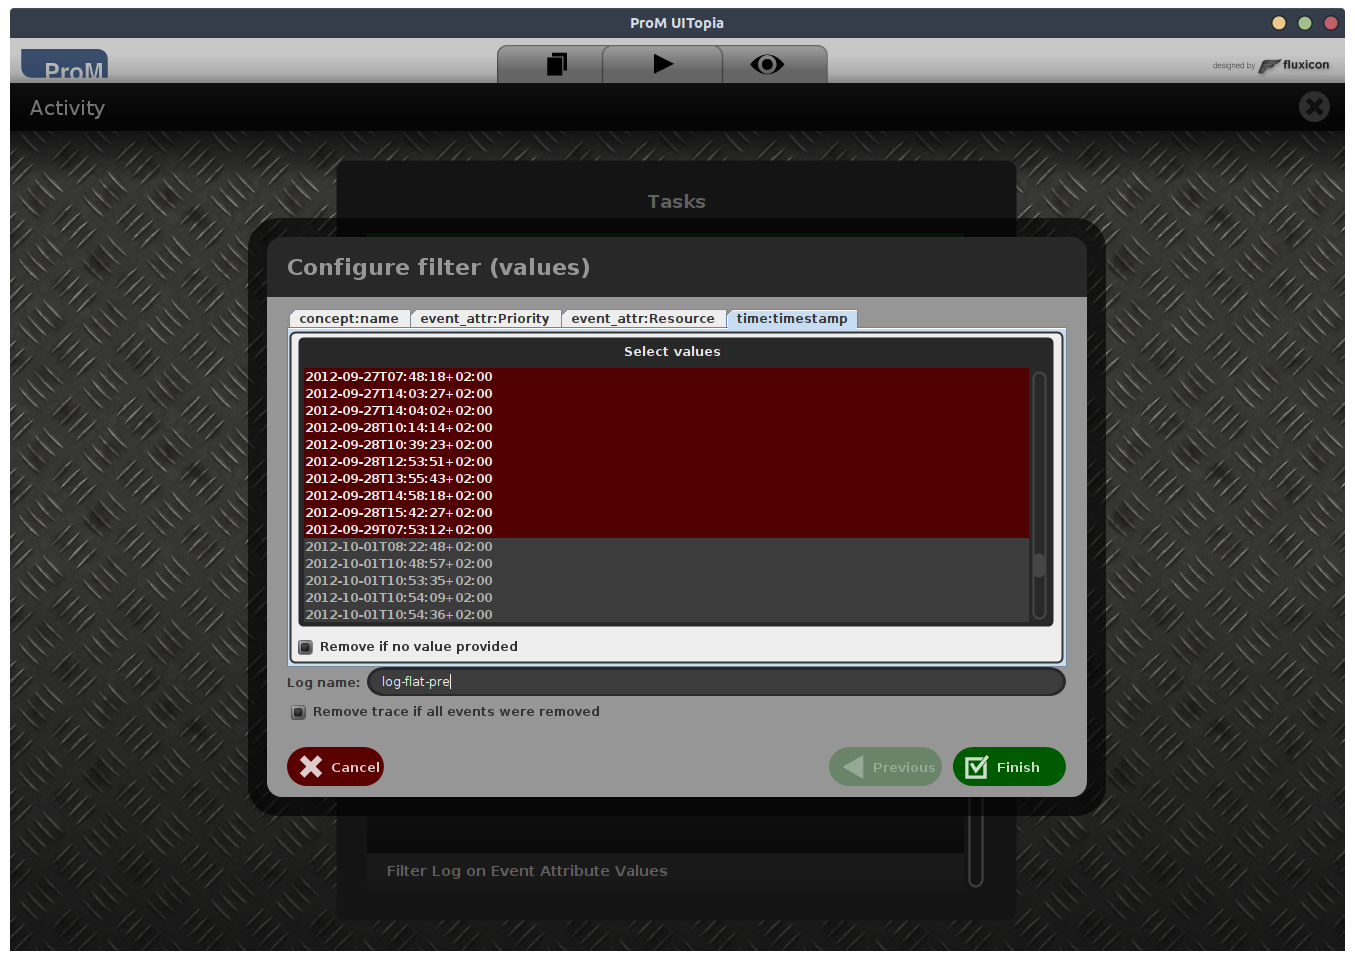
\includegraphics[width=0.33\columnwidth]{img/ProM_a_pre_method.png}
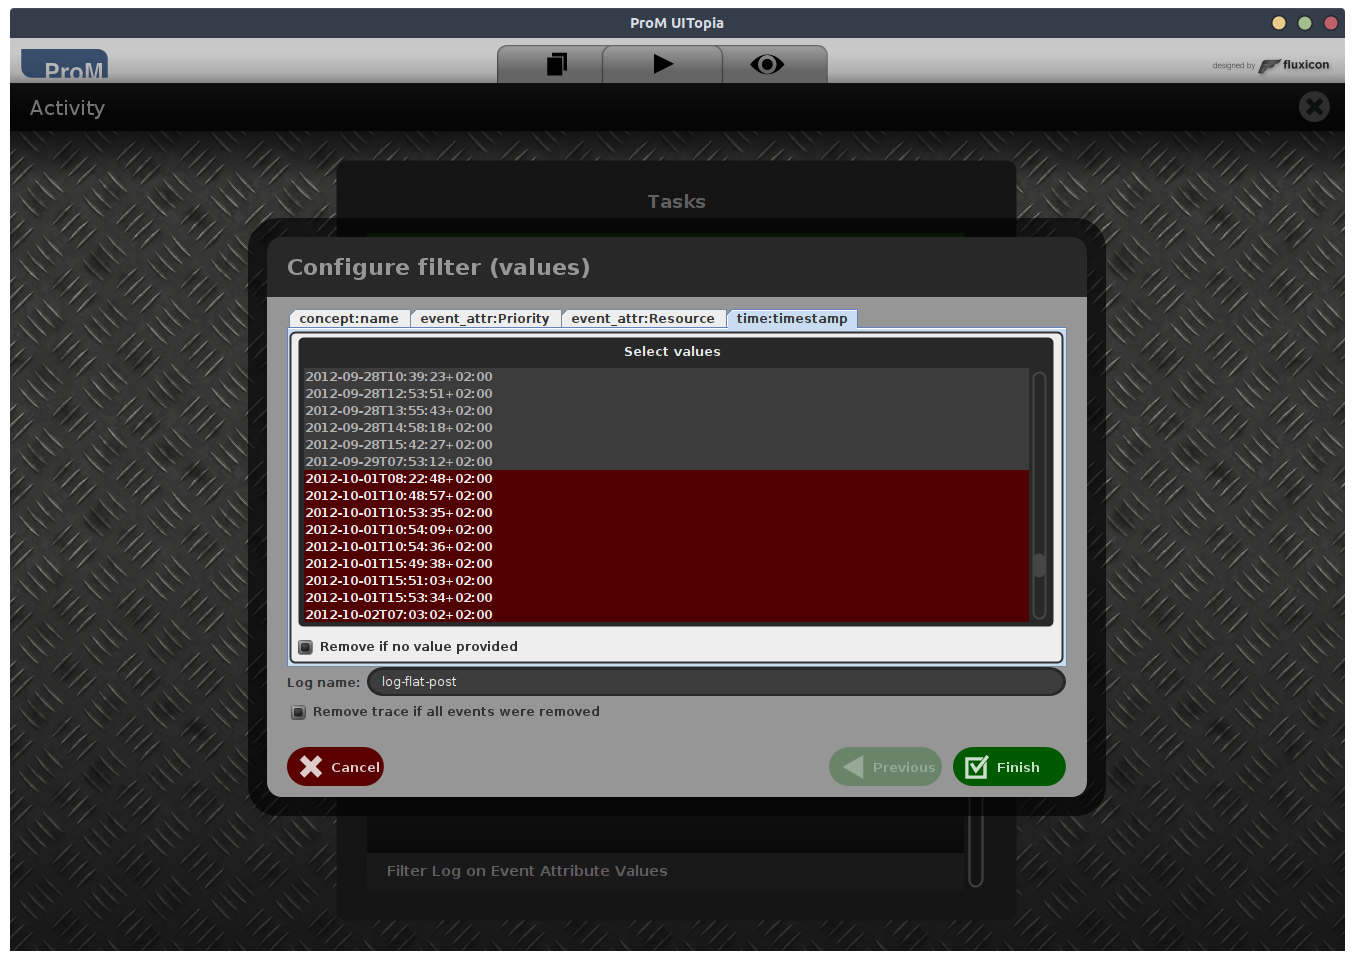
\includegraphics[width=0.33\columnwidth]{img/ProM_a_post_method.png}\\
Afterwards, we can apply our filtering to only allow valid traces, as seen before.\\

For the event log pre 01.10.2012 we get 13 unique activities across 3708 cases, as a whole consisting of 6 variants. \\
For the event log post (including) 01.10.2012 we get 12 unique activities across 730 cases, as a whole consisting of 6 variants. \\
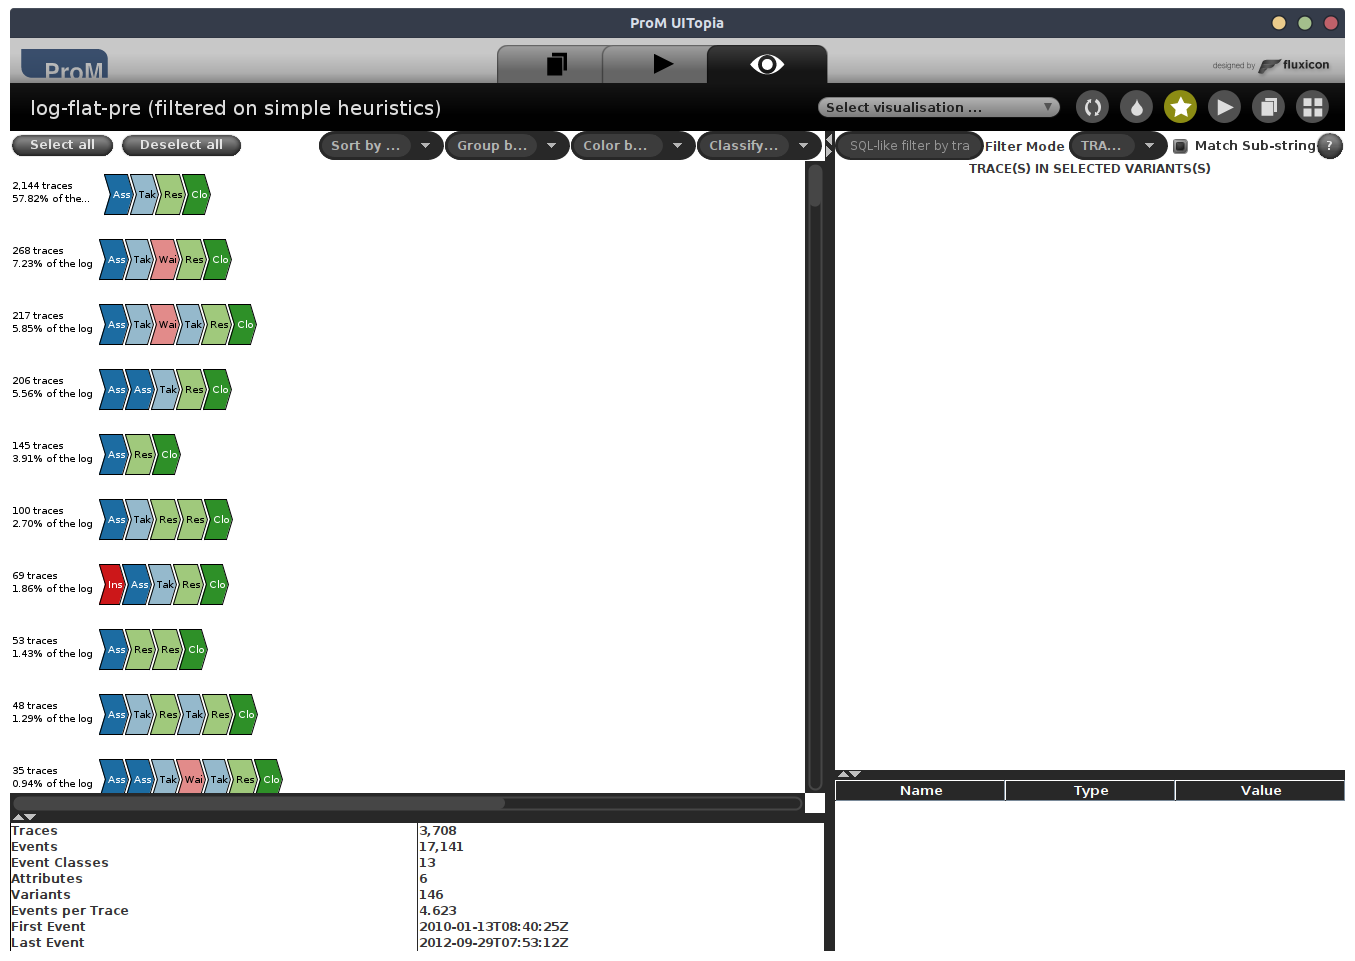
\includegraphics[width=0.5\columnwidth]{img/ProM_a_pre_traces.png}
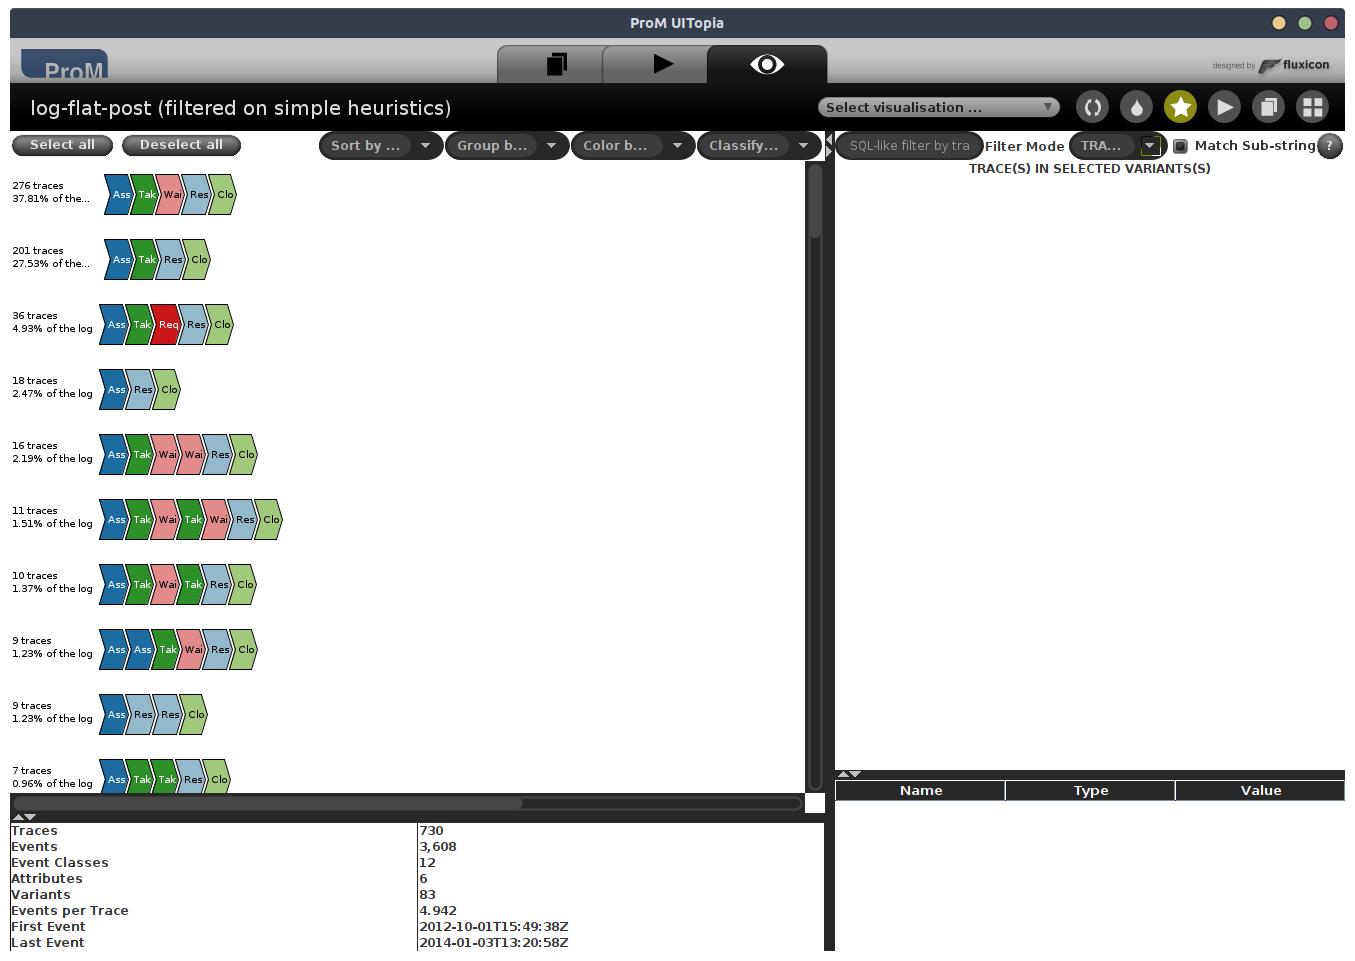
\includegraphics[width=0.5\columnwidth]{img/ProM_a_post_traces.png}\\

\subsection*{(b)}
1. We apply the following workflow both for \textit{log-pre-complete} and \textit{log-post-complete}:
\begin{enumerate}
\item Apply plugin 'Interactive Data-aware Heuristic Miner (iDHM)'
\item Set 'Options \& Thresholds' to\\
\begin{table}[h!]
\begin{tabular}{l|llll}
           & i) (\textit{log-pre-complete}) & ii) (\textit{log-pre-complete}) & iii) (\textit{log-post-complete}) & iv) (\textit{log-post-complete})\\
           \hline
Frequency  & 0.1 & 0   & 0.1  & 0   \\
Dependency & 0.9 & 0.9 & 0.9  & 0.9 \\
Bindings   & 0.1 & 0.1 & 0.1  & 0.1 \\
Conditions & 0.5 & 0.5 & 0.5  & 0.5
\end{tabular}
\end{table}
All tasks connected: True
\item Select 'Petri net' as 'Output: Process Model' and click 'Export model'
\item Use the log and the newly created Petri net as input for the 'Multi-perspective Process Miner' plugin
\end{enumerate}
This results in the following Models:\\
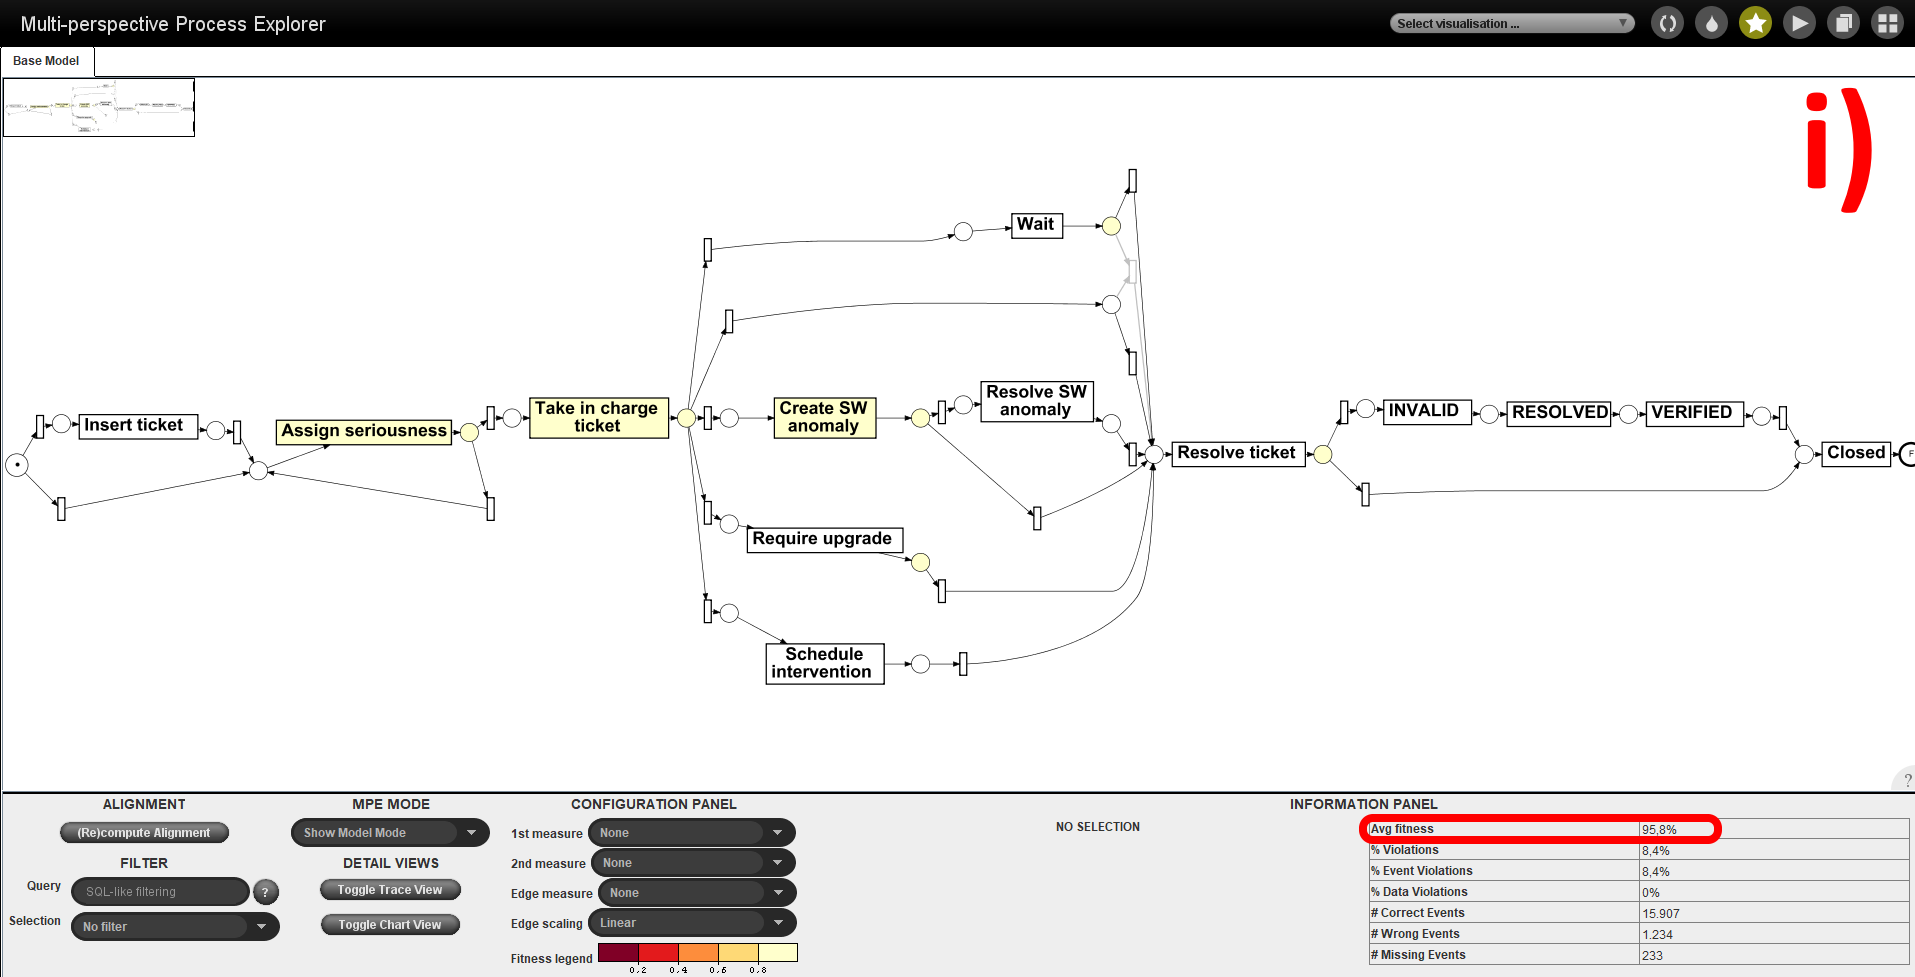
\includegraphics[width=0.5\columnwidth]{img/ProM_b_1i.png}
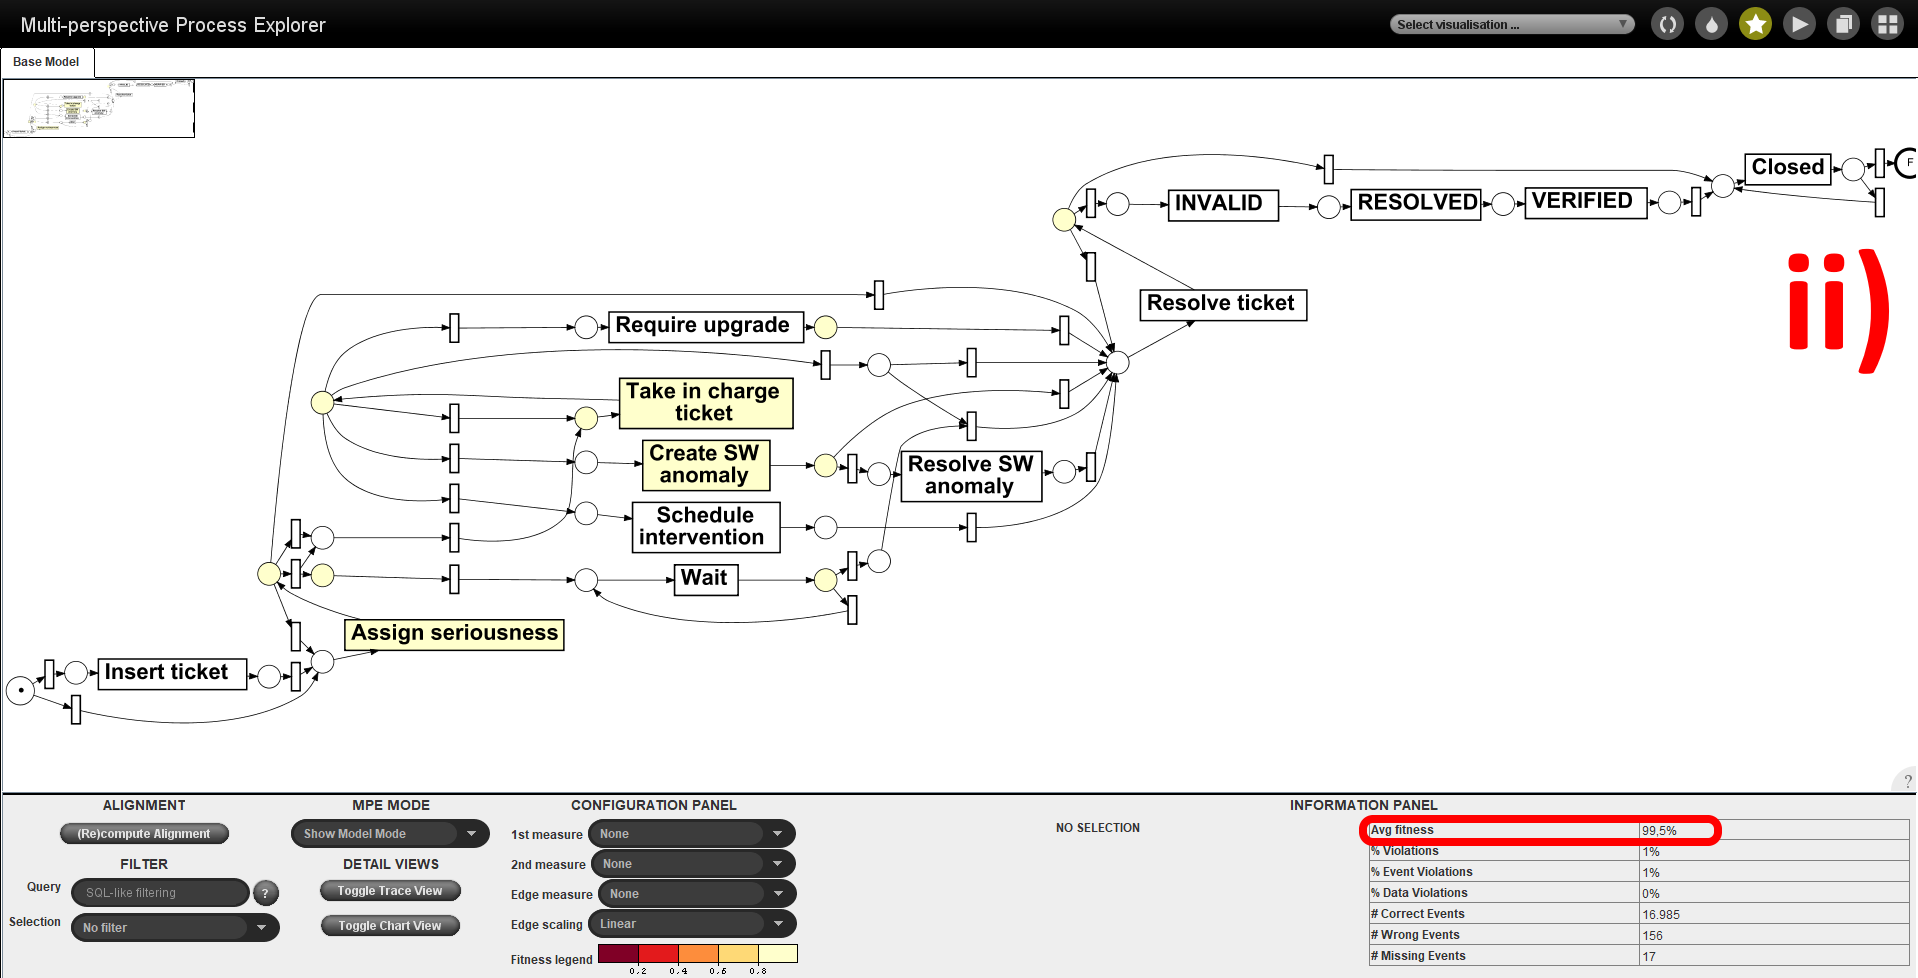
\includegraphics[width=0.5\columnwidth]{img/ProM_b_1ii.png}
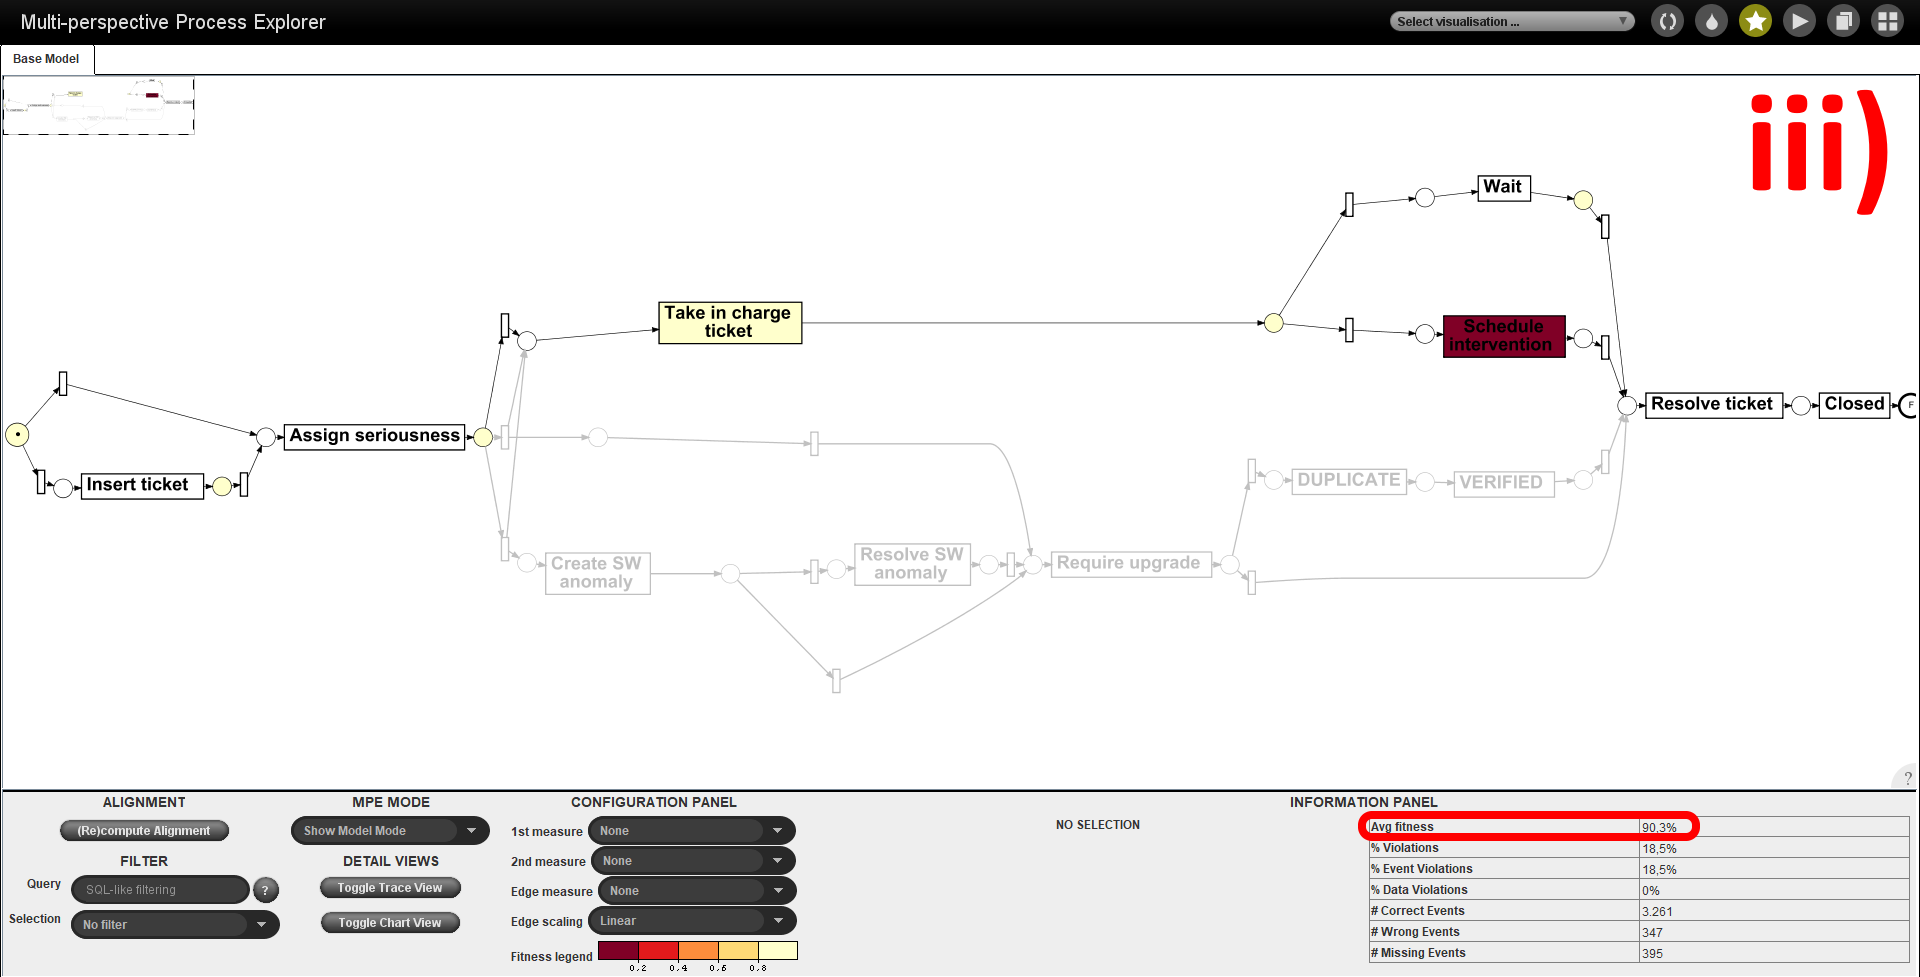
\includegraphics[width=0.5\columnwidth]{img/ProM_b_1iii.png}
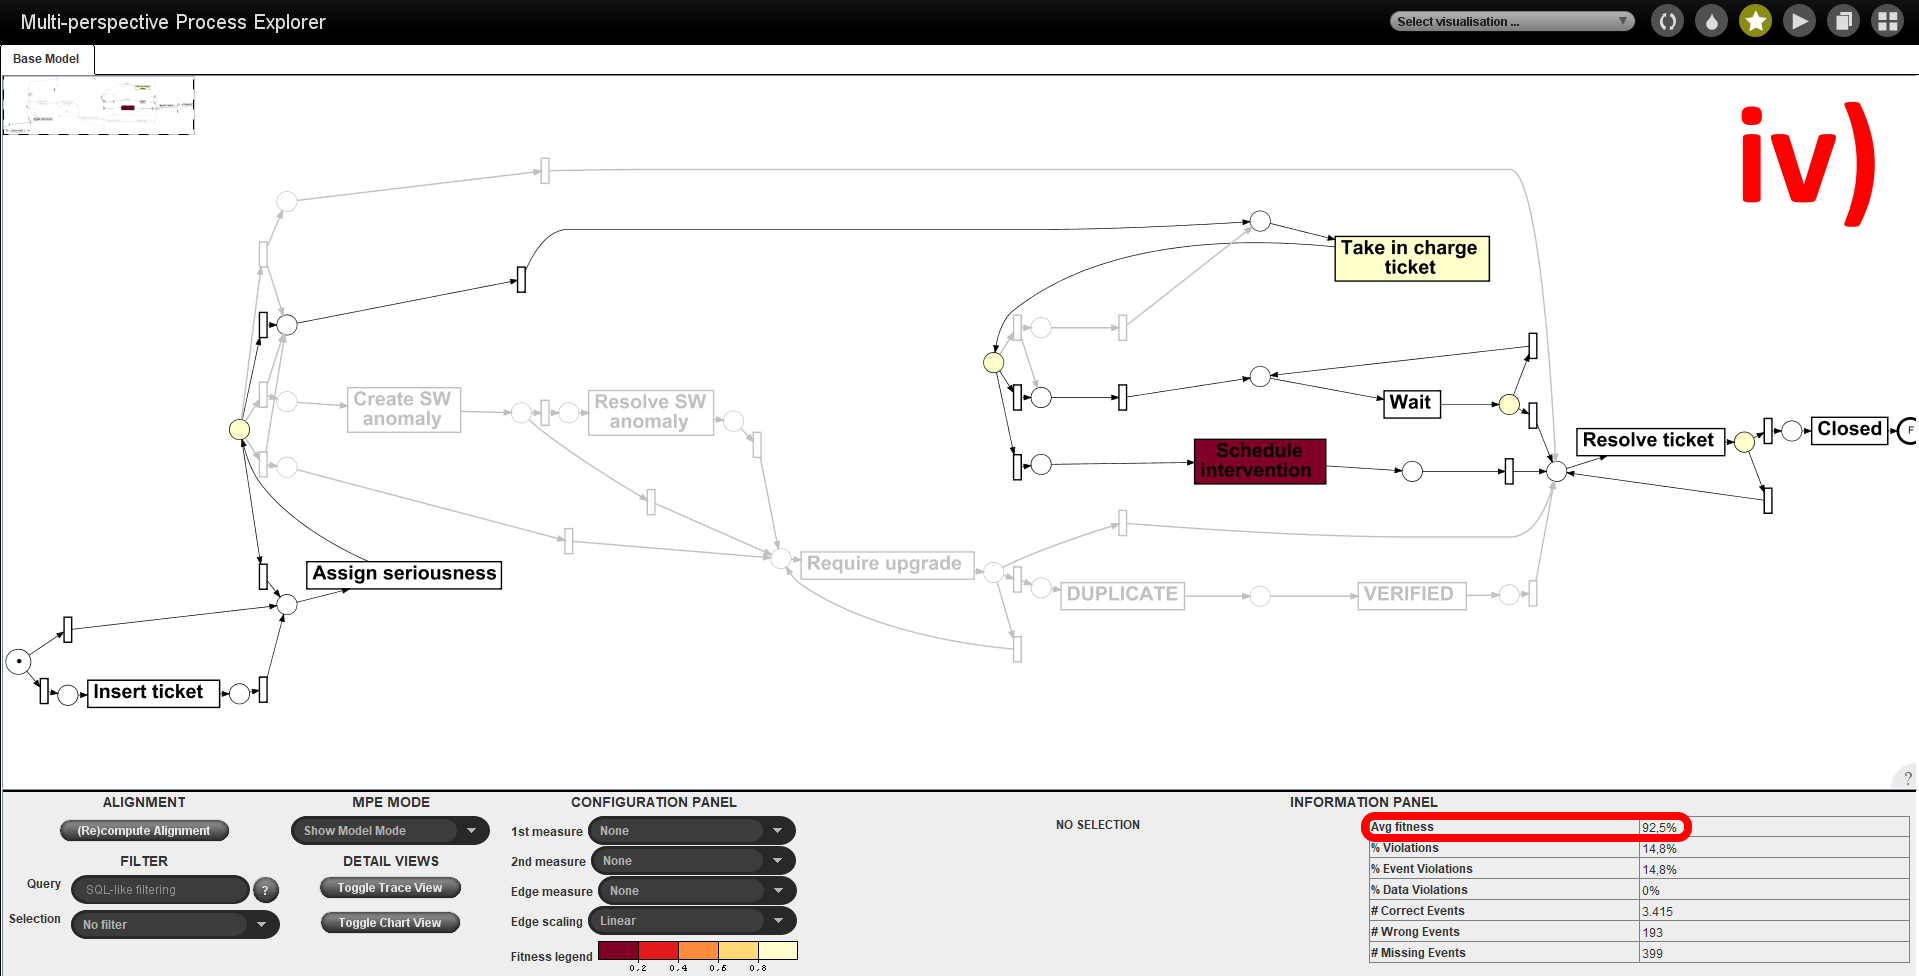
\includegraphics[width=0.5\columnwidth]{img/ProM_b_1iv.png}
As we can see all these models exceed our fitness threshold of 90\% and contain all activities occuring in their respective logs (\textit{log-pre-complete} doesn't contain the activity DUPLICATE and \textit{log-post.complete} doesn't contain the activities INVALID and RESOLVED).

\subsection*{(c)}


\subsection*{(d)}

\end{document}